\documentclass[11pt, english]{article}

\usepackage[T1]{fontenc}
\usepackage{babel}
\usepackage[a4paper, total={6in, 10in}]{geometry}

\usepackage{float}
\usepackage{amsmath}
\usepackage[usenames,dvipsnames]{xcolor}
\usepackage[most]{tcolorbox}
\usepackage{listings} % per scrittura di codice
\usepackage{algorithmic}
\usepackage{algorithm}
\usepackage{booktabs}
\usepackage{multirow}
\usepackage{hyperref}
\hypersetup{
    colorlinks=true,
    linkcolor=blue,
    filecolor=cyan,
    citecolor=blue,
    urlcolor=magenta,
    pdftitle={Overleaf Example},
    pdfpagemode=FullScreen,
    }
\usepackage{footnote}
\usepackage{graphicx}
\graphicspath{{./images}}

\usepackage{biblatex}
\addbibresource{bibliografia.bib}

\definecolor{InlineGray}{HTML}{E3E3E3}

% this style should be active for all lstlistings environments
\lstdefinestyle{all}{
 % columns=flexible,
 tabsize=2,
 columns=fixed,
 keepspaces=true,
 frameshape={}{y}{}{}, % per rimuovere la linea vericale sulla sinistra `frameshape={}{}{}{}`
 basicstyle = {\ttfamily \color{black}},
 showstringspaces=false,
 rulecolor=\color{black},
 numberstyle=\tiny\color{lightgray}
}

\lstdefinestyle{inline}{
 basicstyle={\small\ttfamily \color{black}},
 columns=fixed,
 showstringspaces=false,
}

\tcbset{on line, 
    boxsep=2pt, left=0pt,right=0pt,top=0pt,bottom=0pt,
    colframe=white,colback=InlineGray,
}
\newcommand{\codeinline}[1]{\tcbox{\lstinline[style=inline]|#1|}}

\author{
 Stefanelli Francesco \\
 Matricola 538549\\
 \texttt{fra.stefanelli3@stud.uniroma3.it}
}

\title{\huge\textbf{Report Progetto Deep Learning: Financial Sentiment Analysis }}
\date{\href{https://github.com/Francesco9932/financial-sentiment-analysis}{GitHub: financial-sentiment-analysis}\\ Anno Accademico 2022/2023}



\begin{document}
\maketitle
In questa relazione è stato documentato il lavoro svolto durante lo sviluppo del progetto del corso Deep Learning. Il progetto consiste nell'utilizzare diverse tecniche e modelli di DL per effettuare Sentiment Analysis nel contento delle news finanziarie.
La relazione di divide in tre sezioni: nella prima sezione è riportato il dataset utilizzato per il caso di studio, nella seconda è riportata la fase di preparazione dei dati, nella terza l'implementazione dei modelli utilizzati e nella quarta si presentano i risultati ottenuti e le comparazioni effettuate.

\section{Dataset}
Nella seguente sezione sono illustrati ed analizzati i dataset impiegati per il task di Sentiment Analysis nell'ambito delle news finanziarie. Ciascun dataset sarà composto da: una serie di news headline annotate con il relativo sentiment, che indicherà quanto il titolo finanziario in questione è appetibile da parte di un possibile investitore.

\subsection{FinancialPhraseBank}
Il primo dataset utilizzato allo scopo è stato preso dalla piattaforma Kaggle\footnote{\href{https://www.kaggle.com/datasets/ankurzing/sentiment-analysis-for-financial-news}{Kaggle dataset 1: FinancialPhraseBank}}. Si compone di 4846 news headlines annotate con tre classi (sentiment) e le classi sono rispettivamente positiva (28.1\% sul totale del dataset), negativa (12.5\%) e neutrale (59.4\%).

\begin{figure}[!ht]
    \centering
    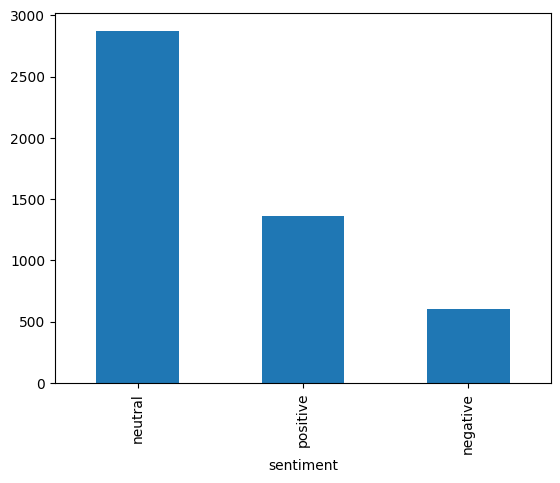
\includegraphics[width=10cm]{./images/dataset_percentage_bar_plot.png}
    \caption{Sample occurencies bar plot per class }
    \label{figure:dataset_perc}
\end{figure}

\subsection{FinancialPhraseBank + FiQA}
Il secondo dataset considerato per l'analisi è un estensione del precente, preso da Kaggle\footnote{\href{https://www.kaggle.com/datasets/sbhatti/financial-sentiment-analysis}{Kaggle dataset 2: FinancialPhraseBank + FiQA}}, che riporta in in totale 5322 news headline annotate nel medesimo modo del precedente dataset. 
Il dataset anche in questo caso si compone di tre classi e sono rispettivamente positiva (31.7\% sul totale del dataset), negativa (14.7\%) e neutrale (53.5\%). Il bilanciamento delle classi, a meno di piccole variazioni percentuali, è lo stesse del precedente dataset. \newline 
Indicate in Figure \ref{figure:dataset_perc}.

\newpage





\section{\label{section:1}Data preparation}
Per la fase di data preparation si è scelto di utilizzare un \textbf{Notebook Jupyter} insieme a \textbf{Python} utilizzando \textbf{Pandas}.
Sono state applicate \codeinline{dropna()} e \codeinline{drop_duplicates()} pre-processing per cancellare le ennuple del dataset contenenti valori nulli e duplicati, la rimozione della punteggiatura e conversione a lowercase. Inoltre, non sono state rimosse le stopwords o effettuate ulteriori fasi di pre-processing dato che sono state ritenute caratteristiche importanti da mantenere per il task di Sentiment Analysis, riuscendo ad ottenere risultati migliori non modificando ulteriormente la frase originale.
Ecco alcuni esempi di news headline dopo la data preparation:
\begin{itemize}
    \item \label{label:1}Positive news headline example : according to the company  s updated strategy for the years 2009 2012   basware targets a long term net sales growth in the range of 20    40   with an operating profit margin of 10    20   of net sales
    \item \label{label:2}Negative news headline example : a tinyurl link takes users to a scamming site promising that users can earn thousands of dollars by becoming a google   nasdaq   goog   cash advertiser
    \item \label{label:3}Neutral news headline example  : technopolis plans to develop in stages an area of no less than 100 000 square meters in order to host companies working in computer technologies and telecommunications   the statement said
\end{itemize}


\section{Modelli e implementazioni}
In questa sezione sono riportate le implementazioni dei vari modelli utilizzati che si basano su due diverse tecniche per la generazione di word embeddings. Entrambe le tecniche conistono in metodi che vanno ad analizzare il testo creando degli embeddings, ovvero delle rappresentazioni compatte delle parole all'interno di uno spazio vettoriale dove due parole simili sono rappresentate da vettori simili. 

\subsection{GloVe}
In particolare la tecnica Global Vectors for Word Representation (GloVe) presentato in \cite{pennington2014glove} si basa sulla tecnica skip-gram e andandone a modificare la loss function introducendone alcune varianti per ridurne la complessità computazionale.
 \subsubsection{Skip-Gram with Global Corpus Statistics}
Si va a denotare con $q_{ij}$ la probabilità condizionata $P({w_{j}} | {w_{i}})$ di una parola contestuale $w_{j}$ data la parola target o centrale $w_{i}$ nel modello skip-gram:
\[q_{ij} = \frac{{\exp(\mathbf{u}_j \cdot \mathbf{v}_i)}}{{\sum_{k=1}^{V} \exp(\mathbf{u}_k \cdot \mathbf{v}_i)}}\]
La formula rappresenta la probabilità condizionata $q_{ij}$, che indica la probabilità che la parola di contesto $j$ si verifichi dato che la parola target $i$ è presente. Nella formula, $\mathbf{u}_j$ rappresenta il vettore di contesto per la parola di contesto $j$, $\mathbf{v}_i$ rappresenta il vettore della parola target $i$, e $\mathbf{u}_k$ rappresenta il vettore di contesto per qualsiasi altra parola $k$ nel corpus. La sommatoria nel denominatore si estende a tutte le parole nel vocabolario $V$ = \{0, 1, 2, \ldots, |V|-1\}.

La parola $w_{i}$ può presentarsi molte volte in un corpus. Tutte le parole contestuali che co-occorrono con wi creano un multiset, dove xij indica il conteggio del numero di volte che la parola wj co-occorre con wi nella stessa finestra di contesto nell'intero corpus. Utilizzando tali statistiche globali del corpus la loss function del modello skip-gram è:
\[-\sum_{i=1}^{V}\sum_{j=1}^{C} x_{ij} \log(q_{ij})\]
Inoltre, si denota con $x_{i}$ il numero delle parole di contesto dove compare $w_{i}$ come parola centrale. Si può definire come la probabilità condizionata $P_{ij} = \frac{x_{ij}}{x_i}$
di generare una parola di contesto $w_{j}$ data una parola centrale $w_{i}$ come:

\[-\sum_{i \in V} x_{i} \sum_{j \in V} p_{ij} \log q_{ij}\]

La sommatoria $-\sum_{j \in V} p_{ij} \log q_{ij}$ è la cross-entropy tra probabilità condizionata $q_{ij}$ relativa alla predizione generata dal modello, e $p_{ij}$ ottenuta analizzando le
statistiche dell'intero corpus.

\subsubsection{Modello GloVe}
Per ridurre la complessità computazionale (soprattutto per generare qij) e per mitigare gli effetti generati dai termini che compaiono di rado nel corpus ma che possono assumere importanza elevata dalla cross entropy, il modello GloVe introduce alcune varianti.


Il modello GloVe (Global Vectors for Word Representation) introduce alcune varianti al fine di ridurre la complessità computazionale e mitigare gli effetti dei termini rari nel corpus ma che potrebbero assumere importanza elevata dalla cross-entropy. I cambiamenti nella loss function consistono in:
\begin{itemize}
    \item Aggiunti due bias, $b_{i}$ per le parole centrali e $c_{i}$ per le parole contetsuali.  
    \item Utilizza delle nuove assegnazioni per evitare di utilizzare la probabilità condizionata $q_{ij}$ modificando la loss e introducendo gli ultimi due termini nel termine al quadrato.
    \item Si rimpiazza il peso di ogni termine della loss con una weight function $h_{x_{ij}}$ che varia nell'intervallo $[0,1]$.
\end{itemize}

Ottenendo come nuova loss function:
\[\sum_{i=1}^{V}\sum_{j=1}^{V} h(x_{ij}) \left( \mathbf{u}_j^T \mathbf{v}_i + b_i + c_j - \log x_{ij} \right)^2\]


  \subsubsection{GloVe - CNN1d}
  L'implementazione con le Convolutional Neural Networks (CNNs) impiega GloVe per generare gli embeddings, una serie di strati conv1D seguiti da GlobalMaxPooling1D e infine alcuni layer MLP con una softmax sull'ultimo strato dense con 3 nodi pari al numero di classi in output. Il dettaglio è indicato in Table \ref{tab:cnn}.

\begin{table}[!ht]
\centering
\caption{GloVe-CNN1d detailed model architecture}
\label{tab:cnn}
\begin{tabular}{ccccc}
\toprule
Layer & Maps & Kernel size & Activation & Dropout prob.\\
\midrule
    GloVe Embedding & - & - & - & - \\
    Convolution1d & 200 & 2x2 & ReLU & -\\
    GlobalMaxPooling1D & 200 & - & - & -\\
    Convolution1d & 200 & 3x3 & ReLU & -\\
    GlobalMaxPooling1D & 200 & - & - & -\\
    Convolution1d & 200 & 4x4 & ReLU & -\\
    GlobalMaxPooling1D & 200 & - & - & -\\
    Convolution1d & 200 & 5x5 & ReLU & -\\
    GlobalMaxPooling1D & 200 & - & - & -\\
    Convolution1d & 200 & 6x6 & ReLU & -\\
    GlobalMaxPooling1D & 200 & - & - & -\\
    Concatenate & 1000 & - & - & -\\
    Dropout & - & - & - & 0.1\\
    Fully Connected & 128 & - & ReLU & -\\
    Dropout & - & - & - & 0.2\\
    Fully Connected & 3 & - & Softmax & -\\
\bottomrule
\end{tabular}
\end{table}
\newpage

  \subsubsection{GloVe - LSTM}
  Anche l'implementazione con la Long short-term memory (LSTM) impiega GloVe per generare gli embeddings, successivamemte un layer ricorrente LSTM, un layer di flatten e infine alcuni layer MLP con una softmax sull'ultimo strato dense con 3 nodi pari al numero di classi in output. Nel dettaglio:
\begin{table}[!ht]
\centering
\caption{GloVe-LSTM detailed model architecture}
\begin{tabular}{cccc}
\toprule
Layer & Nodes & Return sequences & Activation \\
\midrule
    GloVe Embedding & - & - & - \\
    LSTM & 256 & True & TanH \\
    Flatten & - & - & - \\
    Fully Connected & 3 & - & Softmax\\
\bottomrule
\end{tabular}
\end{table}
  
\newpage

\subsection{BERT}
Il modello BERT proposto in \cite{devlin2019bert} per la generazione degli word embeddings combina due approcci differenti: 
\begin{itemize}
    \item \textit{Context-Indipendent}: data una parola, il vettore generato non dipenderà dal contesto attuale per cui termini polisemici o relazioni semantiche del linguaggio naturale saranno ignorate.
    \item \textit{Context-sensitive}: si combinano le rappresentazioni intermedie per ottenere una rappresentazione che dipende dalla sequenza in input.
\end{itemize}
BERT rappresenta l'intero contesto mediante un approccio bidirezionale e si basa su un architettura encoder-decoder di trasformers pre-addestrati su auxiliary task. Dell'intera architettura transformers verrà utilizzata però solamente l'encoder dato che l'obiettivo di questo modello è quello di generare un language model. 
In particolare in input c'è un singolo testo o una coppia di testi, che permette di andare a definire due auxiliary task differenti su cui è stata pre-addestrata la rete sui cui poi sarà possibile effettuare fine-tuning in base al contesto specifico. \newline
Un primo auxiliary task chiamato \textit{Next Sentence Prediction} consiste nel prendere coppie di testi e far predire alla rete se la seconda frase in coppia  è la frase successiva nel documento originale. Durante l'addestramento, il 50\% degli input è una coppia in cui la seconda frase è la frase successiva nel documento originale, mentre nell'altro 50\% viene scelta una frase random dal corpus come seconda frase. L'assunzione si basa sul fatto che la frase casuale sia slegata dalla prima frase.
\newline
Alla coppia di frasi si si aggiungono in fase di tokenizzazione due special token, rispettivamente \textit{CLS} inserito all'inizio della frase e \textit{SEP} inserito alla fine di ogni farse e poi successivamente viene sommato il sentence embedding che andrà a rappresentare se si la frase in questione è la frase A o la frase B. I due embedding così descritti verranno poi sommati ai positional embedding classici di un'architettura transformers, rappresentanti la posizione di un termine rispetto agli altri in una certa frase.\newline
Per andare poi a predire se la seconda frase è effettivamente collegata alla prima l'intera sequenza in input viene passata all'interno del modello e tramite uno strato di classificazione binaria insieme ad una softmax come funzione di attivazione si ottiene la predizione.
\newline
Dal modello pre-addestrato su questo auxiliary task appena descritto si è andato poi ad effettuare fine-tuning per il task obiettivo del progetto, ovvero la Sentiment Analysis.
Un ulteriore auxiliary task utile in altri contesti su cui gli autori di BERT hanno pre-addestrato il modello è il \textit{Masked Language Modeling}, dove dato un corpus testuale il 15\% dei tokens saranno selezionati in modo random per il task di predizione e al loro posto sarà presente un tag [mask].

\begin{figure}[!ht]
    \centering
    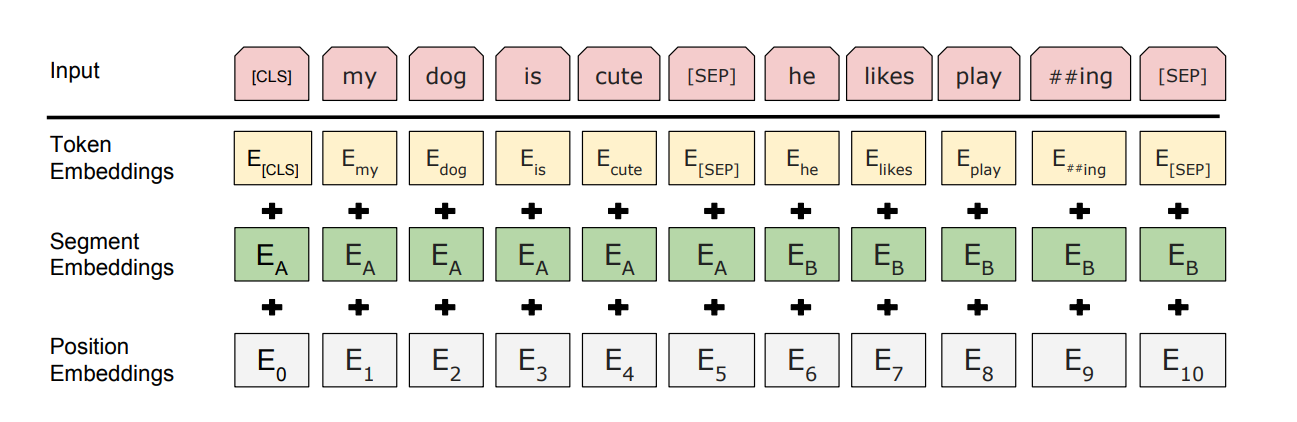
\includegraphics[width=15cm]{./images/bert.png}
    \caption{BERT input representation}
\end{figure}

\newpage
Nel seguito verranno riportate le versioni pretrained e le implementazioni utilizzate per il caso d'uso.\newline
Su entrambe le versioni di BERT l'implementazione della classe wrapper realizzata con Tensorflow è la seguente:
\begin{table}[!ht]
\centering
\caption{BERT Wrapper detailed model architecture}
\begin{tabular}{cccc}
\toprule
Layer & Maps & Dropout prob. & Activation \\
\midrule
    Pretrained BERT layer & - & - & - \\
    GlobalMaxPooling1D & 768 & - & - \\
    Fully Connected & 128 & - & ReLU\\
    Dropout & - & 0.1 & - \\
    Fully Connected & 32 & - & ReLU\\
    Fully Connected & 3 & - & Softmax\\
\bottomrule
\end{tabular}
\end{table}


\subsubsection{FinBERT}
FinBERT \cite{araci2019finbert} è una versione su cui è stato effettuato ulteriore pre-training della versione base di BERT. Gli autori di questa versione, FinBERT, hanno ulteriormente addestrato la rete su un corpus di dati finanziari per effettuare anche Sentiment Analysis, il dataset che hanno utilizzato gli autori è il Financial PhraseBank, lo stesso dataset utilizzato nella presente. 
Il modello pre-addestrato di FinBERT utilizzato nel training e nella valutazione del modello è quello offerto dalla libreria HuggingFace.\footnote{\href{https://huggingface.co/ProsusAI/finbert}{Pretrained HuggingFace FinBERT from ProsusAI}}  

    
\subsubsection{DistilBERT}
DistilBERT \cite{sanh2020distilbert} è una versione più piccola, veloce e leggera di BERT base. Ha il 40\% in meno di parametri rispetto a bert-base-uncased, funziona il 60\% più velocemente, preservando al contempo oltre il 95\% delle prestazioni di BERT misurate sul benchmark di comprensione del linguaggio GLUE. Il modello pre-addestrato di DistilBERT utilizzato nel training e nella valutazione del modello è stato sempre preso da HuggingFace.\footnote{\href{https://huggingface.co/distilbert-base-uncased}{Pretrained HuggingFace distilbert-base-uncased}}  



% https://towardsdatascience.com/bert-explained-state-of-the-art-language-model-for-nlp-f8b21a9b6270

% https://arxiv.org/pdf/1810.04805.pdf 

\section{Risultati}
In questa sezione sono riportati i risultati ottenuti in termini di metriche fondamentali, la pipeline seguita per il training, evalutaion dei modelli e i grafici a confronto dell'andamento dell'accuracy su train e validation set durante l'addestramento. Il dettaglio verrà approfondito nella sezione apposita. 

\subsection{Configurazione Software/Hardware}
La configurazione con il quale sono stati effettuati i test è \textbf{Google Colab} utilizzando come tipo di runtime: Python3; Acceleratore hardware: GPU; Tipo di gpu: T4. Per l'implementazione, training dei modelli e valutazione dei modelli è stato utilizzato \textbf{Tensorflow} 2.12.0. La libreria utilizzata per i modelli preaddestrati di BERT è \textbf{Transformers} 4.29.2 di HuggingFace. Infine, \textbf{Sklearn} 1.2.2 per il preprocessing, train-test split e calcolo delle metriche.  

\subsection{Valutazione dei modelli}
\subsubsection{Metriche di valutazione}
Per la valutazioni dei modelli sono state utilizzate le metriche di Precision (Eq. \ref{eq:precisione}), Recall (Eq. \ref{eq:richiamo}), F1-Score (Eq. \ref{eq:f1_score}) e Accuracy (Eq. \ref{eq:accuracy}).
\begin{equation}
P = \frac{TP}{TP+FP} \label{eq:precisione}
\end{equation}

\begin{equation}
R = \frac{TP}{TP+FN} \label{eq:richiamo}
\end{equation}

\begin{equation}
\text{F1-Score} = 2 \times \frac{\text{Precision} \times \text{Recall}}{\text{Precision} + \text{Recall}} \label{eq:f1_score}
\end{equation}

\begin{equation}
\text{Accuracy} = \frac{TP + TN}{TP + TN + FP + FN} \label{eq:accuracy}
\end{equation}

\subsubsection{Comparazione e Training dei modelli}
Dopo aver effettuato il preprocessing dei dataset e la definizione dei modelli come da capitoli precenti la pipeline che si è andato a seguire 
(compresa anche di data preparation) è descritta in Figure \ref{fig:pipeline}.

\begin{figure}[!ht]
    \centering
    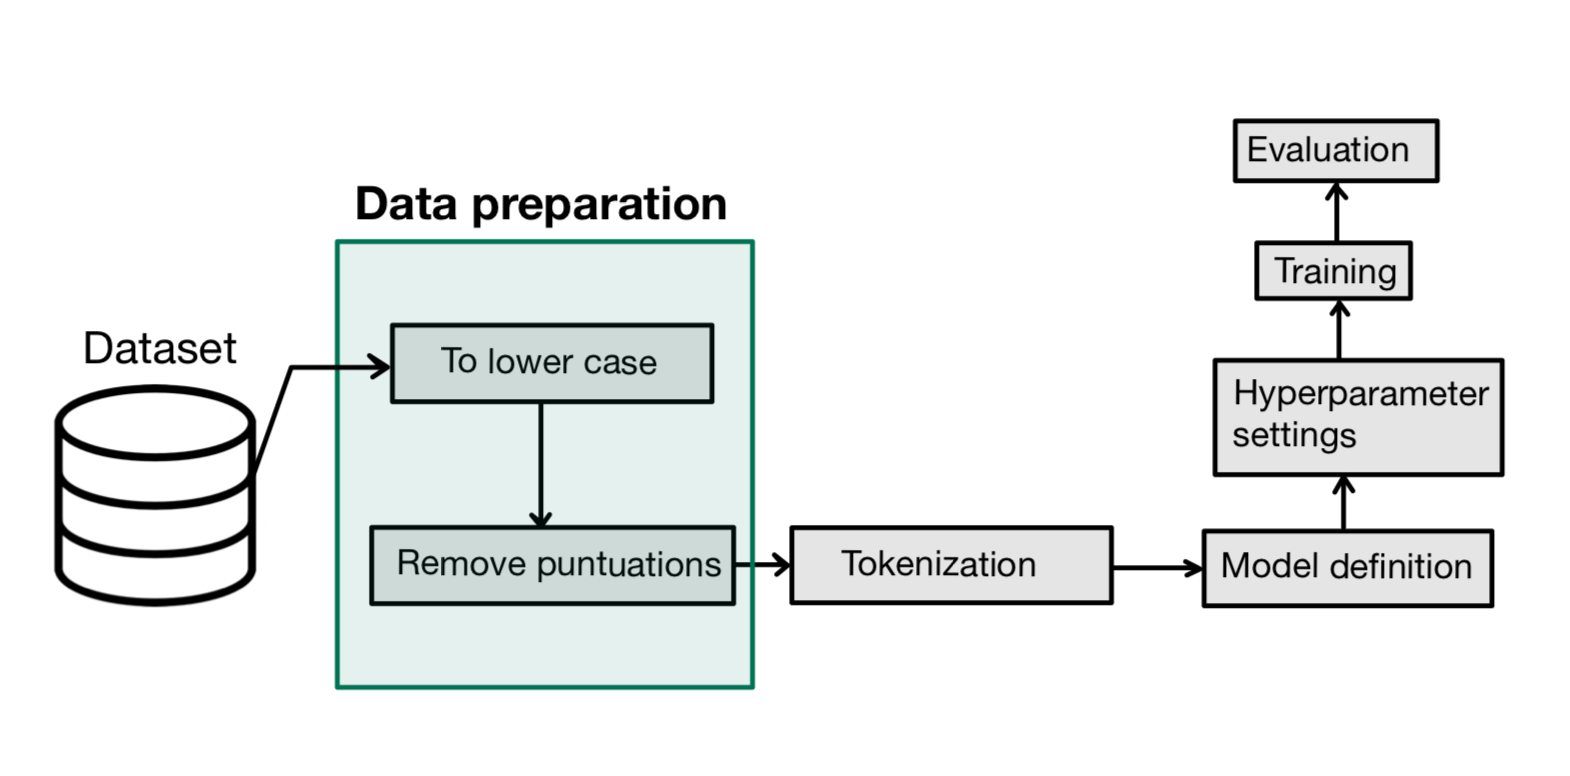
\includegraphics[width=12cm]{./images/pipeline.png}
    \caption{Implemented pipeline for Financial Sentiment Analysis}
    \label{fig:pipeline}
\end{figure}
\newpage
Inoltre la suddivisione in train-val-test set del dataset segue queste percentuali:
\begin{itemize}
    \item Train set: 70\%
    \item Validation set: 10\% del train set
    \item Test set: 30\%
\end{itemize}
Per il training di tutti e 4 i modelli impiegati nello studio del caso di studio sono state utilizzate due callbacks per cercare di evitare l'overfitting dei modelli durante il training, rispettivamente: early stopping e model checkpoint. Il model checkpoint  è stato impostato tale per cui andrà a salvare la versione del modello con la validation accuracy più alta durante il training. Mentre, l'early stopping terminerà il training se la validation accuracy non è migliorata per un numero di volte pari al parametro di patience.
L'optimizer utilizzato per tutti e 4 i modelli è Adam, dove per i modelli GloVe based sono stati utilizzati i parametri di default di Keras, mentre per le versioni di BERT il learning rate (lr) è pari a 5 $\times 10^{-5}$, $\epsilon = 1 \times 10^{-8}$ e clipnorm $= 1.0$.
Tutti gli altri iperparametri di training e le callbacks nello specifico sono indicate in Table \ref{tab:hyper-parameter}.
\newline
Infine, in Table \ref{tab:performance1}, \ref{tab:performance2} si possono vedere i valori, per entrambi i dataset considerati, di precision, recall e f1-score ottenuti in fase di validazione dei modelli. Tali valori sono stati presi tramite il metodo \codeinline{classificationReport()} di Sklearn, riportando come valori quelli con macroAVG, ovvero mediati sul numero delle classi. 

\begin{table}[!ht]
  \centering
  \begin{tabular}{c|c|c|c|c|c|c|c|c}
    Methods & Opimizer & Loss & Metric & Batch Size & Epochs & ES Patience\\
    \midrule
    GloVe+CNN & Adam & Sparse CCE & Accuracy & 32 & 100 & 5 \\
    GloVe+LSTM & Adam & Sparse CCE & Accuracy & 32 & 100 & 5\\
    FinBERT & Adam & CCE & Accuracy & 32 & 10 & 3\\
    DistilBERT & Adam & CCE & Accuracy & 32 & 10 & 3\\
    \bottomrule
  \end{tabular}
  \caption{Hyperparameters and compiling details of used methods}
  \label{tab:hyper-parameter}
\end{table}

\begin{table}[!ht]
  \centering
  \begin{tabular}{c|c|c|c|c}
    Methods & Precision (\%) & Recall (\%) & F1-Score (\%) & Accuracy (\%) \\
    \midrule
    GloVe+CNN & 77.38 & 73.47 & 75.14 & 79.27 \\
    GloVe+LSTM & 72.60 & 70.82 & 71.21 & 75.76 \\
    FinBERT & \textbf{84.52} & \textbf{83.22} & \textbf{83.82} & \textbf{85.54} \\
    DistilBERT & 84.49 & 81.14 & 82.66 & 84.44 \\
    \bottomrule
  \end{tabular}
  \caption{Performance comparization of implemented models on FinancialPhraseBank dataset}
  \label{tab:performance1}
\end{table}

\begin{table}[!ht]
  \centering
  \begin{tabular}{c|c|c|c|c}
    Methods & Precision (\%) & Recall (\%) & F1-Score (\%) & Accuracy (\%) \\
    \midrule
    GloVe+CNN & 63.76 & 60.84 & 61.28 & 73.22 \\
    GloVe+LSTM & 61.18 & 57.51 & 57.77 & 69.16 \\
    FinBERT & \textbf{72.11} & \textbf{74.45} & \textbf{73.07} & \textbf{78.18} \\
    DistilBERT & 69.60 & 68.58 & 68.97 & 76.47 \\
    \bottomrule
  \end{tabular}
  \caption{Performance comparization of implemented models on FinancialPhraseBank+FiQA dataset}
  \label{tab:performance2}
\end{table}

\newpage

\subsubsection{Grafici Training/Val Accuracy dei modelli su FinancialPhraseBank}
Come nella precedente sottosezione anche qui sono riportati i grafici della training/val accuracy dei vari modelli sul dataset FinancialPhraseBank.\newline
Rispettivamente del modello GloVe+CNN1d:
\begin{figure}[!ht]
    \centering
    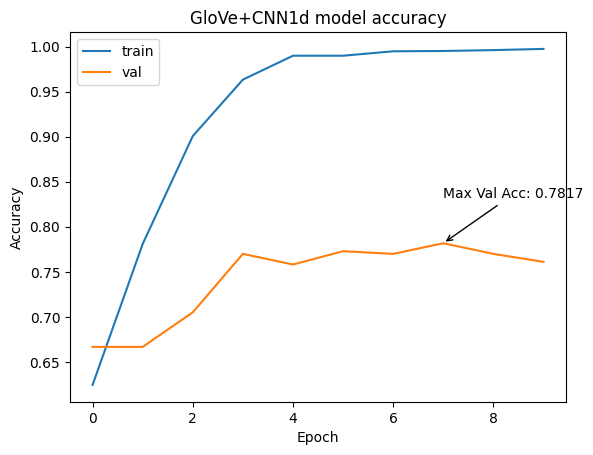
\includegraphics[width=12cm]{./images/plot_cnn.png}
    \caption{Plot of GloVe+CNN1d train/val accuracy}
\end{figure}
\newline
GloVe+LSTM:
\begin{figure}[!ht]
    \centering
    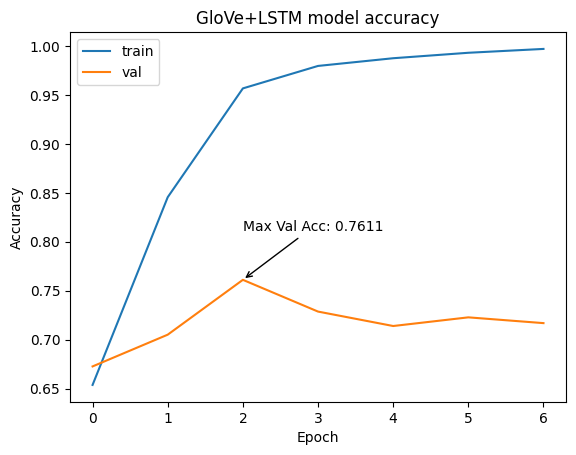
\includegraphics[width=11.5cm]{./images/plot_lstm.png}
    \caption{Plot of GloVe+LSTM train/val accuracy}
\end{figure}
\newline
\newpage
finBERT:
\begin{figure}[!ht]
    \centering
    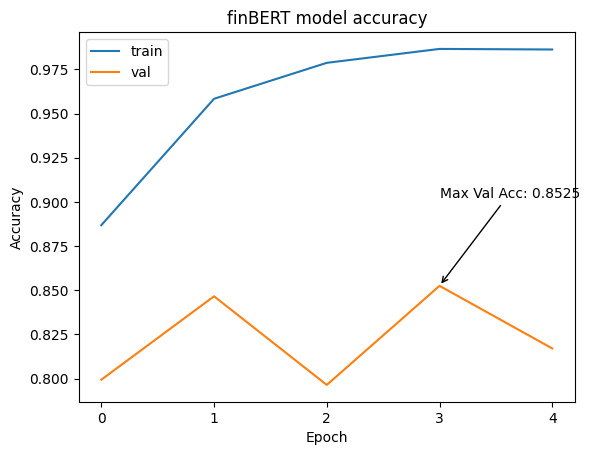
\includegraphics[width=12cm]{./images/plot_finBERT.png}
    \caption{Plot of FinBERT train/val accuracy}
\end{figure}
\newline
distilBERT:
\begin{figure}[!ht]
    \centering
    \includegraphics[width=12cm]{./images/plot_distilBERT.png}
    \caption{Plot of DistilBERT train/val accuracy}
\end{figure}

\newpage

\subsubsection{Grafici Training/Val Accuracy dei modelli su FinancialPhraseBank+FiQA}
Come nella precedente sottosezione anche qui sono riportati i grafici della training/val accuracy dei vari modelli sul dataset FinancialPhraseBank+FiQA.\newline
Rispettivamente del modello GloVe+CNN1d:
\begin{figure}[!ht]
    \centering
    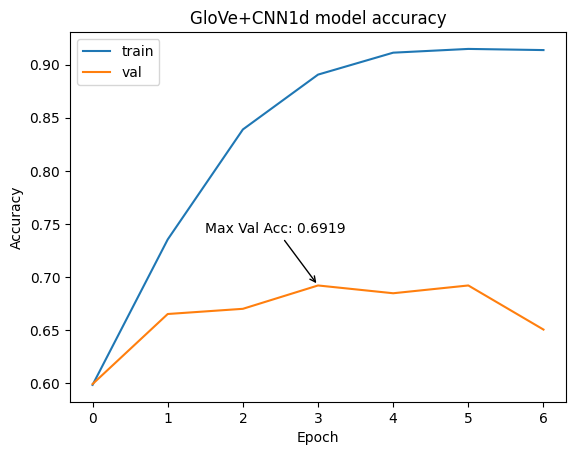
\includegraphics[width=12cm]{./images/acc_glove_cnn_2.png}
    \caption{Plot of GloVe+CNN1d train/val accuracy}
\end{figure}
\newline
GloVe+LSTM:
\begin{figure}[!ht]
    \centering
    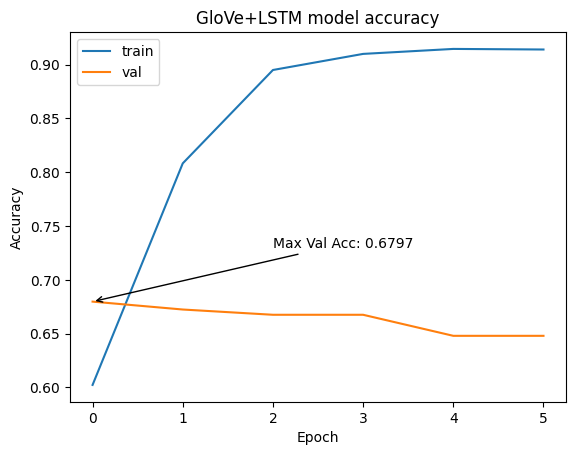
\includegraphics[width=11.5cm]{./images/acc_glove_lstm_2.png}
    \caption{Plot of GloVe+LSTM train/val accuracy}
\end{figure}
\newline
\newpage
finBERT:
\begin{figure}[!ht]
    \centering
    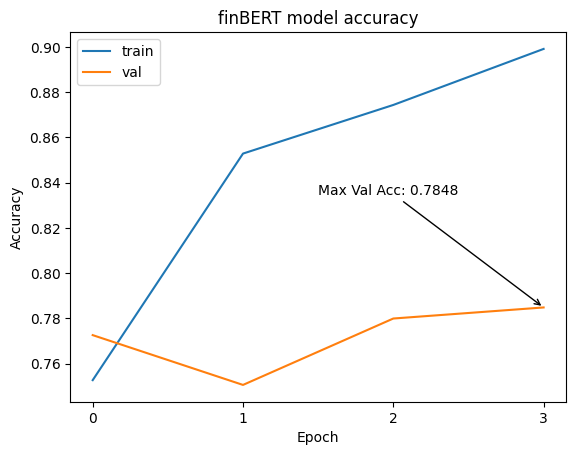
\includegraphics[width=12cm]{./images/acc_finBERT_2.png}
    \caption{Plot of FinBERT train/val accuracy}
\end{figure}
\newline
distilBERT:
\begin{figure}[!ht]
    \centering
    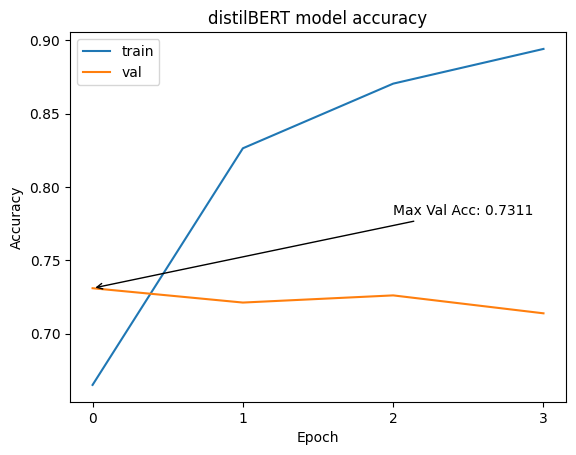
\includegraphics[width=12cm]{./images/acc_distilBERT_2.png}
    \caption{Plot of DistilBERT train/val accuracy}
\end{figure}

\newpage

\subsection{Output}
Di seguito sono riportate le previsioni ottenute in output dai relativi modelli sulle headline prese in esempio in \ref{section:1}:
    \begin{table}[!ht]
    \centering
    \caption{Example prediction of GloVe+CNN}
    \begin{tabular}{ccc}
      \toprule
          Headline &  Prediction & True label \\
          \midrule
          Positive news headline \ref{label:1} & neutral & positive \\
          Negative news headline & neutral & negative \\
          Neutral news headline & neutral & neutral \\
          \bottomrule
    \end{tabular}
  \end{table}

    \begin{table}[!ht]
    \centering
    \caption{Example prediction of GloVe+LSTM}
    \begin{tabular}{ccc}
      \toprule
          Headline &  Prediction & True label \\
          \midrule
          Positive news headline \ref{label:1} & positive & positive \\
          Negative news headline & negative & negative \\
          Neutral news headline & neutral & neutral \\
          \bottomrule
    \end{tabular}
  \end{table}

\begin{table}[!ht]
    \centering
    \caption{Example prediction of FinBERT}
    \begin{tabular}{ccc}
      \toprule
          Headline &  Prediction & True label \\
          \midrule
          Positive news headline \ref{label:1} & positive & positive \\
          Negative news headline & negative & negative \\
          Neutral news headline & neutral & neutral \\
          \bottomrule
    \end{tabular}
  \end{table}

  \begin{table}[!ht]
    \centering
    \caption{Example prediction of DistilBERT}
    \begin{tabular}{ccc}
      \toprule
          Headline &  Prediction & True label \\
          \midrule
          Positive news headline \ref{label:1} & positive & positive \\
          Negative news headline & negative & negative \\
          Neutral news headline & neutral & neutral \\
          \bottomrule
    \end{tabular}
  \end{table}
\newpage





\printbibliography[title={Riferimenti}]




\end{document}